\documentclass[tikz,border=6mm]{standalone}

\usepackage[T1]{fontenc}
\usepackage[scaled=0.92]{helvet}
\renewcommand{\familydefault}{\sfdefault}

\usepackage{amsmath}
\usepackage{tikz}
\usetikzlibrary{arrows.meta,positioning,calc,shadows.blur,fit,shapes.geometric}

\begin{document}

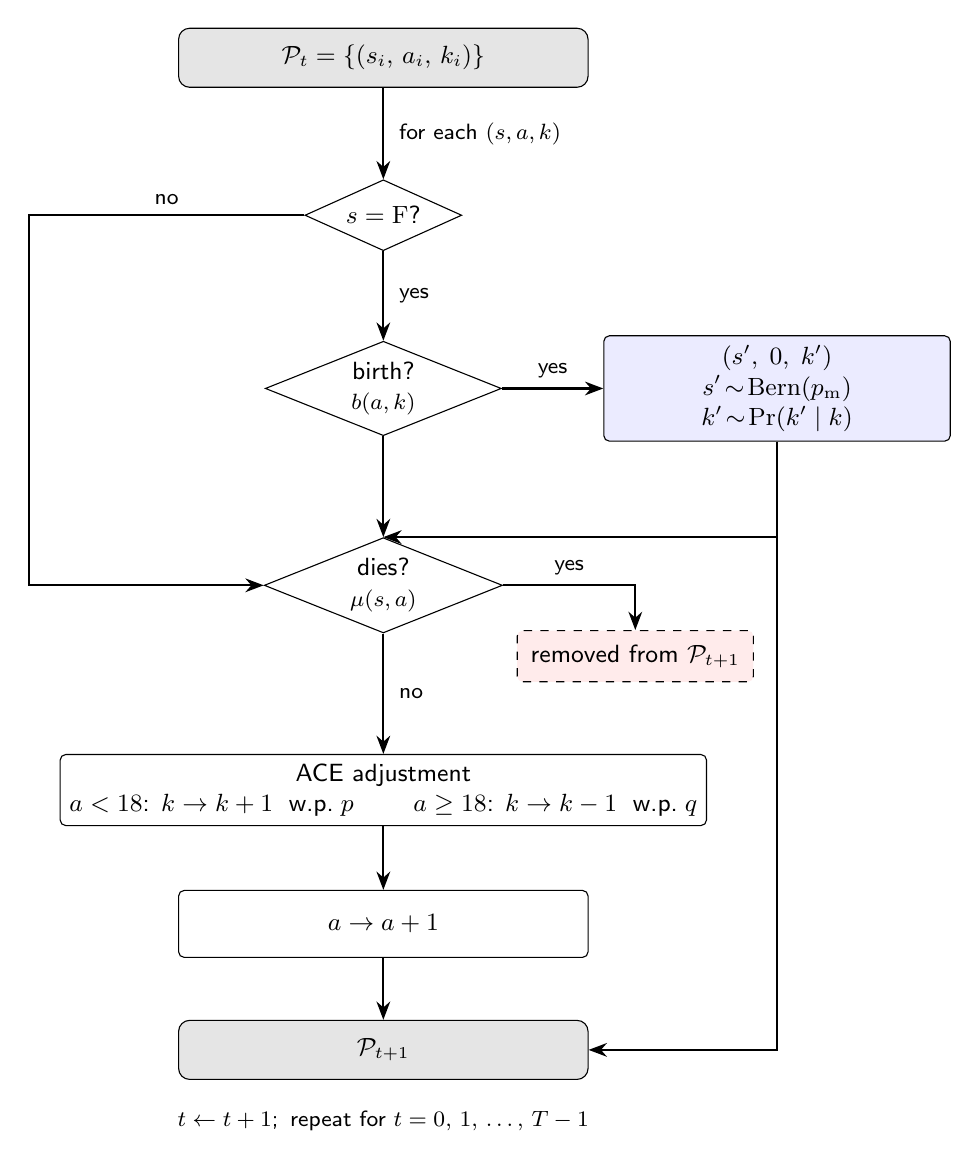
\begin{tikzpicture}[
  pop/.style={
    rectangle, draw, rounded corners=4pt, fill=gray!20,
    minimum width=5.2cm, minimum height=0.75cm,
    align=center, font=\small\bfseries},
  proc/.style={
    rectangle, draw, rounded corners=2pt, fill=white,
    minimum width=5.2cm, minimum height=0.85cm,
    align=center, font=\small},
  dec/.style={
    diamond, draw, aspect=2.5, fill=white,
    minimum height=0.9cm, align=center,
    font=\small, inner sep=2pt},
  newborn/.style={
    rectangle, draw, rounded corners=2pt, fill=blue!8,
    minimum width=4.4cm, minimum height=1.0cm,
    align=center, font=\small},
  gone/.style={
    rectangle, draw, dashed, rounded corners=2pt, fill=red!8,
    minimum width=3.0cm, minimum height=0.65cm,
    align=center, font=\small},
  arr/.style={-Stealth, thick},
  lbl/.style={font=\footnotesize},
]

%% ---- Nodes ----
\node[pop]     (pt)    at (0,    0  ) {$\mathcal{P}_t = \{(s_i,\, a_i,\, k_i)\}$};

\node[dec]     (fem)   at (0,   -2.0) {$s = \mathrm{F}$?};

\node[dec]     (birth) at (0,   -4.2) {birth?\\\footnotesize$b(a,k)$};
\node[newborn] (child) at (5.0, -4.2) {$(s',\;0,\;k')$\\
                                        $s'\!\sim\!\mathrm{Bern}(p_{\mathrm{m}})$\\
                                        $k'\!\sim\!\Pr(k'\mid k)$};

\node[dec]     (death) at (0,   -6.7) {dies?\\\footnotesize$\mu(s,a)$};
\node[gone]    (dead)  at (3.2, -7.6) {removed from $\mathcal{P}_{t+1}$};

\node[proc]    (aces)  at (0,   -9.3) {ACE adjustment\\
  $a < 18$: $k \to k+1$ \;w.p.\;$p$ \qquad
  $a \geq 18$: $k \to k-1$ \;w.p.\;$q$};

\node[proc]    (age)   at (0,  -11.0) {$a \to a + 1$};

\node[pop]     (pt1)   at (0,  -12.6) {$\mathcal{P}_{t+1}$};

%% ---- Main flow ----
\draw[arr] (pt.south)    -- node[lbl, right=2pt] {for each $(s,a,k)$} (fem.north);
\draw[arr] (fem.south)   -- node[lbl, right=2pt] {yes} (birth.north);
\draw[arr] (birth.south) -- (death.north);
\draw[arr] (death.south) -- node[lbl, right=2pt] {no} (aces.north);
\draw[arr] (aces.south)  -- (age.north);
\draw[arr] (age.south)   -- (pt1.north);

%% ---- Right branches ----
\draw[arr] (birth.east) -- node[lbl, above] {yes} (child.west);
    \draw[arr] (death.east) -- node[lbl, above] {yes} (death.east -| dead.north) -- (dead.north);

%% ---- Female ``no'' branch: goes left then down then east into death ----
\draw[arr] (fem.west) -- node[lbl, above] {no} ++(-3.5,0)
    |- (death.west);

%% ---- Child feeds into P_{t+1} ----
\draw[arr] (child.south) -- (child.south |- pt1.east) -- (pt1.east);
\draw[arr] (child.south) -- (child.south |- death.north) -- (death.north);

%% ---- Iteration note ----
\node[lbl, align=center] at (0,-13.5)
    {$t \leftarrow t+1$;\enspace repeat for $t = 0,\,1,\,\dots,\,T-1$};

\end{tikzpicture}

\end{document}
